\documentclass[tikz,border=2pt]{standalone}
\usepackage{amsmath,amssymb}
\usepackage{tikz}
\usetikzlibrary{arrows.meta}

\begin{document}
% Euler tour algorithm: follow unused edges from s until you are back at s (cycle Omega,
% blue); from a vertex of Omega that still has unused edges start a second cycle (red) and
% splice it into Omega.
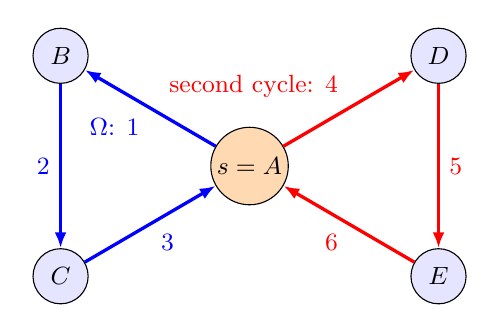
\begin{tikzpicture}[every node/.style={font=\small}, >={Latex[length=2mm]}, v/.style={draw, circle, fill=blue!10, minimum size=7mm, inner sep=0pt}]
	\node[v, fill=orange!30, inner sep=1.5pt] (A) at (0,0) {$s=A$};
	\node[v] (B) at (-2.4,1.4) {$B$};
	\node[v] (C) at (-2.4,-1.4) {$C$};
	\node[v] (D) at (2.4,1.4) {$D$};
	\node[v] (E) at (2.4,-1.4) {$E$};
	\draw[blue, very thick, ->] (A) -- (B) node[midway, below left] {$\Omega$: 1};
	\draw[blue, very thick, ->] (B) -- (C) node[midway, left] {2};
	\draw[blue, very thick, ->] (C) -- (A) node[midway, below right] {3};
	\draw[red, very thick, ->] (A) -- (D) node[midway, above left] {second cycle: 4};
	\draw[red, very thick, ->] (D) -- (E) node[midway, right] {5};
	\draw[red, very thick, ->] (E) -- (A) node[midway, below left] {6};
	\end{tikzpicture}
\end{document}
